\documentclass{article}
\usepackage{geometry}
\geometry{a4paper, margin=1in}
\usepackage{array}
\usepackage{graphicx}
\usepackage{lastpage}
\usepackage{hyperref}
\usepackage{fancyhdr}  % For custom headers and footers

\title{Problemformulering \\ \large PROJ3-Gruppe-4}

\pagestyle{fancy}      % Use fancy page style
\fancyhf{}             % Clear all headers and footers
\fancyfoot[C]{\thepage\ af \pageref{LastPage}} % Sidetal af total antal sider

\begin{document}
% Forside
\begin{titlepage}
    \centering
    \vspace*{4cm}
    {\Huge \textbf{Problemformulering}} \\[1cm]
    {\Large \textbf{PROJ3-SW Gruppe 4}} \\[1cm]
    {\large Dato: \today}\\[0.5cm]
    \textbf{Forfattere:} \\[0.2cm]
    \begin{center}
        \begin{tabular}{|c|c|c|}
            \hline
            \textbf{Navn:} & \textbf{ID:} \\
            \hline
            Lucas Foged Bugge Stilborg & 202307401 \\
            \hline
            Sanne Yding Feddersen  & 202004994 \\
            \hline
            Kevin Nguyen  & 202304713 \\
            \hline
            Rene Sand Schumacher  & 202305367 \\
            \hline
            Magnus Hvidsten Christiansen & 202007772 \\
            \hline
            Lasse Fink Hansen & 202306755\\
            \hline
            Jakob Alsina Lund & 202308406 \\
            \hline
            Simon Bøjgård Nowack & 202308256\\
            \hline
            Fillip Fontao & 202109701\\
            \hline
        \end{tabular}
    \end{center}
    \textbf{Versionshistorik:} \\[0.2cm]
    \begin{center}
        \begin{tabular}{|c|c|c|c|}
            \hline
            \textbf{Version:} & \textbf{Dato:} & \textbf{Initialer:} & \textbf{Beskrivelse:} \\
            \hline
            1.0 & 18/09/2024 & Fælles & Første version af problemformulering lavet i fælleskab \\
            \hline
        \end{tabular}
    \end{center}
    \vfill
    \begin{center}
        \begin{tabular}{|c|c|c|}
            \hline
            \textbf{Version:} & 1.0 \\
            \hline
        \end{tabular}
    \end{center}
\end{titlepage}


\newpage

Mangel på kvalitetsrig søvn er et gennemgående problem for mange mennesker. En dårlig søvn gør ikke kun en træt, det påvirker også en masse andre parametre. Øget stressniveau, nedsat koncentrationsevne og svækket immunforsvar er blot nogle af de mange negative konsekvenser, som dårlig søvn indebærer. Et eksperiment i 2018 er kommet frem til, at 41\% af danskere sover dårligt og uroligt. Det anbefales, at den gennemsnitlige person sover 7-9 timer pr. nat, men dette er ikke den eneste forudsætning for en god søvn. Gennem research er man kommet frem til en række faktorer, som spiller ind i kvaliteten af søvn, blandt andet søvnstadie, støj i omgivelser osv. Det er dog begrænset, hvor meget indsigt den gennemsnitlige person har i sin egen søvn.

Formålet med projektet er at skabe og udvikle et system, SleepMaxx, der tackler disse problemstillinger. SleepMaxx vil anvende en række sensorer, der samlet skal kunne give en evaluering af den pågældende søvn:

\begin{itemize}
    \item En mikrofon der skal observere snorken og støj i rummet.
    \item En bevægelsessensor der skal måle uroligheder i løbet af natten.
    \item Pulsmålere da en persons puls under søvn kan være med til at give et indblik i søvnkvalitet.
    \item EEG-teknologi - dette vil omfatte elektroder, der skal kunne observere hvilket søvnstadie brugeren befinder sig i. Her kan der også beregnes, hvornår det optimale interval for at vække brugeren ville være.
\end{itemize}

Udover at indsamle data om brugerens søvnkvalitet skal SleepMaxx også kunne vække brugeren. Derfor implementeres der yderligere en højtaler, der skal fungere som en alarm. Denne alarm skal kunne indstilles gennem en brugergrænseflade, som er tilknyttet systemet.

SleepMaxx er tiltænkt de personer, som ønsker at optimere deres søvn for at være den bedste version af dem selv. Derfor vil brugerfladen også kunne fremvise data for den observerede søvn og samtidig komme med anbefalinger til optimering af søvn baseret på de resultater, som systemet er kommet frem til.

Til udførelse af projektet vil der gøres brug af en PSoC. Denne mikrocontroller har til formål at styre højtaleren og samtlige sensorer og dertil indsamle data fra disse. Derudover anvendes en Raspberry Pi som interface til PSoC, og den skal samtidig agere som grænseflade, som brugeren kan interagere med.

Det ønskes, at SleepMaxx kan integreres med andre IoT-enheder for yderligere at optimere systemets funktionalitet. Det kunne indebære en glidende overgang af lysniveau vha. automatisk lys- og gardinregulering. 

Alt dette skal medføre en optimering af brugerens søvn- og dermed livskvalitet.

\begin{figure}[h!]
    \centering
    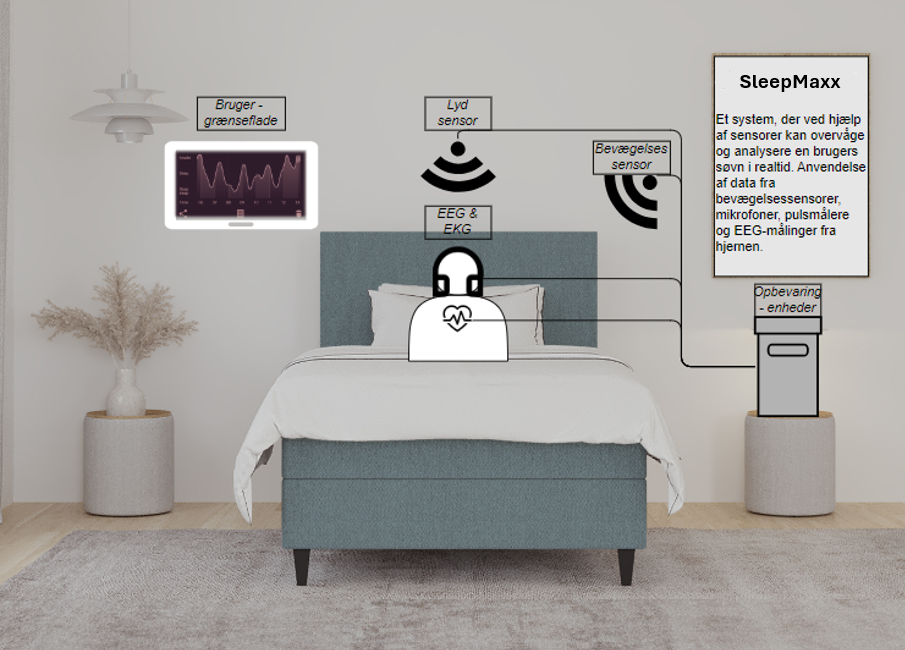
\includegraphics[width=1\textwidth]{SleepMaxx_image.png}
    \caption{SleepMaxx systembillede}
    \label{fig:sleepmaxx}
\end{figure}

\end{document}
